%----------------------------------------------------------------------------------------
%
% A LaTeX-template for 1DV510. Modified and translated by Björn Lindenberg at LNU.
% Based on an original master thesis template created by Marcus Wilhelmsson at LNU.
%
%----------------------------------------------------------------------------------------

% Settings and document configuration

\documentclass[a4paper,12pt]{article} 
\usepackage[T1]{fontenc} 
\usepackage{times} 
\usepackage[swedish,english]{babel} 
\usepackage[utf8]{inputenc} 
\usepackage{dtk-logos} 
\usepackage{wallpaper} 
\usepackage[absolute]{textpos} 
\usepackage[top=2cm, bottom=2.5cm, left=3cm, right=3cm]{geometry} 
\usepackage[parfill]{parskip} 
\usepackage{csquotes} 
\usepackage{float} 
\usepackage{lipsum} % Used for dummy text. Can be removed.
\usepackage{hyperref}
\hypersetup{
    colorlinks=true,
    linkcolor=black,
    filecolor=magenta,      
    urlcolor=blue,
    citecolor= black,
}
\usepackage[nottoc]{tocbibind}
% Fontsizes for section headings.
\usepackage{sectsty} 
\sectionfont{\fontsize{14}{15}\selectfont}
\subsectionfont{\fontsize{12}{15}\selectfont}
\subsubsectionfont{\fontsize{12}{15}\selectfont}

%----------------------------------------------------------------------------------------
%	This part is used for the text box on the title page
%----------------------------------------------------------------------------------------
\newsavebox{\mybox}
\newlength{\mydepth}
\newlength{\myheight}

\newenvironment{sidebar}%
{\begin{lrbox}{\mybox}\begin{minipage}{\textwidth}}%
{\end{minipage}\end{lrbox}%
 \settodepth{\mydepth}{\usebox{\mybox}}%
 \settoheight{\myheight}{\usebox{\mybox}}%
 \addtolength{\myheight}{\mydepth}%
 \noindent\makebox[0pt]{\hspace{-20pt}\rule[-\mydepth]{1pt}{\myheight}}%
 \usebox{\mybox}}

%----------------------------------------------------------------------------------------
%	Title
%----------------------------------------------------------------------------------------
\newcommand\BackgroundPic{
    \put(-2,-3){
    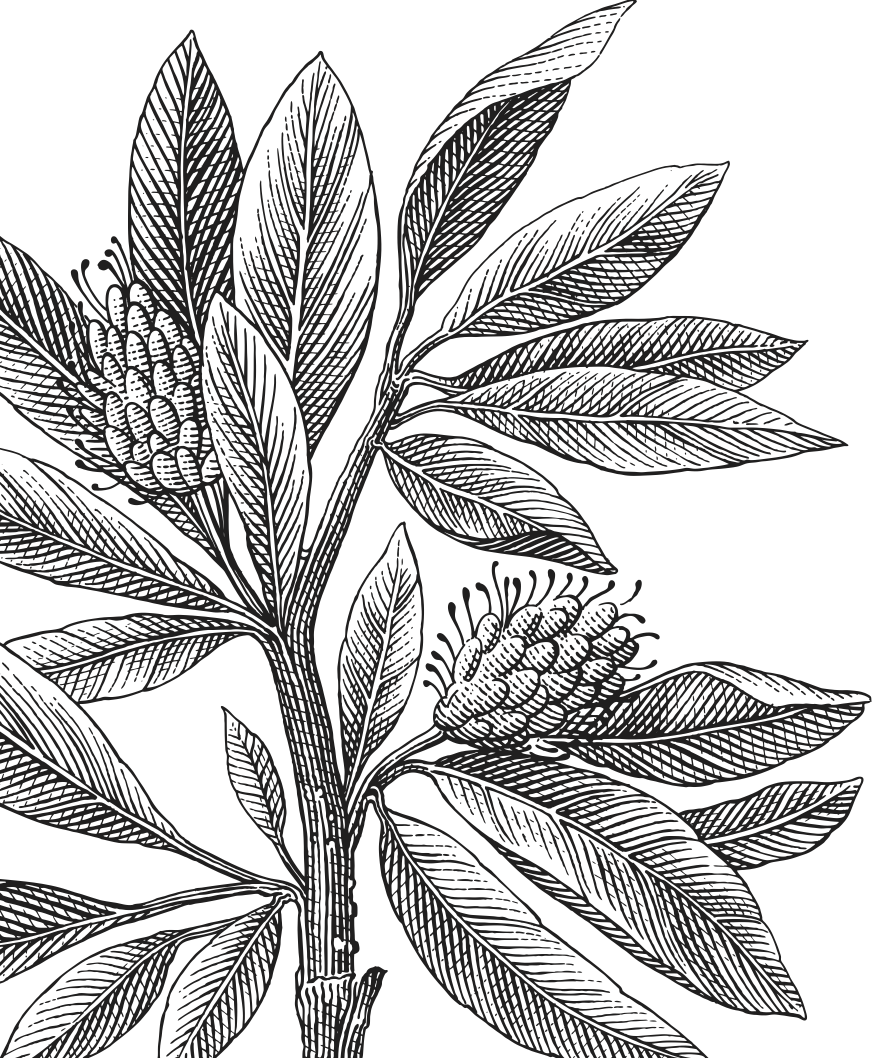
\includegraphics[keepaspectratio,scale=0.3]{img/lnu_etch.png} % Background image
    }
}
\newcommand\BackgroundPicLogo{
    \put(30,740){
    
\includegraphics[keepaspectratio,scale=0.10]{img/logo.png} % LNU logo
    }
}

\title{
\vspace{-8cm}
\begin{sidebar}
    \vspace{10cm}
    \normalfont \normalsize
    \huge Report\\ % Main title
    \vspace{-1.3cm}
\end{sidebar}
\vspace{3cm}
\begin{flushleft}
    \huge Act I: The University Server \\% Subtitle
    \emph{Date: 14/03/2021}
\end{flushleft}
\null
\vfill
\begin{textblock}{6}(10,13)
\begin{flushright}
\begin{minipage}{\textwidth}
\begin{flushleft} \large
\emph{Author:}  Anas \textsc{Kwefati}\\  % Author
\emph{Email:} ak223wd@student.lnu.se\\ %Email
\emph{Semester:} Spring 2021\\ % Semester
\emph{Area:} Digital Forensics \\ % Area
\emph{Course code:} 2DV704 % Course
\end{flushleft}
\end{minipage}
\end{flushright}
\end{textblock}
}

\date{} % Empty date command. Use \today inside for today's date.
\author{} % Normally one would use this to define authors. However in this case the title command takes care of everything, so we leave the field empty to get rid of warnings. 

\begin{document}

\pagenumbering{gobble} % Turn off page numbering
\newgeometry{left=5cm}
\AddToShipoutPicture*{\BackgroundPic} % Adds the background image to the title page
\AddToShipoutPicture*{\BackgroundPicLogo} % Adds the logo to the title page
\maketitle % Prints the title
\restoregeometry
\clearpage

\pagenumbering{roman} % Roman page numbering for abstract page


\newpage

\pagenumbering{gobble} % Turn off page numbering
\tableofcontents 

\newpage
\pagenumbering{arabic} % Turn on page numbering

% Some example sections with dummy text
\section{Executive Summary}
\label{exe}

%This portion of the report will provide a synopsis of the purpose of the examination and the investigator’s major findings. In law enforcement, a separation of duties often occurs, particularly in larger computer forensics labs. This means that one officer works the investigation, and another officer performs the forensic analysis.
%
%Therefore, the work of more than one law enforcement agent is included in the report, and that must be clearly outlined in the report.

The University has contacted us for an investigation that would confirm if the professor Bob lab's server was infected with a worm or not. This issue has been notified, and suspected by the Network Operations Center (NOC), saying that his lab's server was infected with a worm, due to a huge spike in Internet traffic at 4 in the morning. 
This professor seems to not think it was infected, however, because the University was eager to obtain an independent confirmation, they had to contact us. According to the professor, there were no many files except on his own account called "bob". Other accounts might have files, such as "eric", "kevin", "peter", and "takeda". 

\section{Purpose of the Investigation}

%This section is optional because the report writer may have explained the reason for conducting the investigation in the Executive Summary. To set the tone for the report, the report writer might want to explain the reason for the investigation and the scope of the warrant, which will later help explain the types of computing devices that were examined and the areas of memory that were analyzed. For example, picture and video files will be important in a suspected pedophile case, whereas emails might be particularly important in a corporate insider investigation, and bank information is important in an embezzlement investigation.

The reason for conducting the investigation can be read in Section \ref{exe}. But to sum it up, the university has contacted us, due to a notification from NOC saying that a university server has been compromised due to a huge spike in Internet traffic at 4 a.m. Hence, in that case, we will probably check, if there are any malware in the hard disk, then verify the logs section of the image to see if anything happened. We have managed to obtain the server image, and we are investing it using Kali Linux 2020.3 in a Virtual Machine environment.

\section{Methodology}

%The methodology can be included as a separate section in the report or can be included later. The methodology explains the science behind the examination. It should explain the approach the forensics examiner took, which might include the choice of software or hardware tools. The investigator may also reference standard practices for computer forensics examinations that were used in the examination—these could be lab specific, could come from the Department of Justice, or could be recommendations from NIST.

In this Forensic examination, we have decided to download \textbf{act1.img}, in our local computer using the command tool rsync. Then, we mounted that image into our Kali Linux VM using VirtualBox. We decided to use Kali Linux as it regroups many tools that can be used for digital forensics. Before actually mounting the image, we made sure to keep a copy of the image, and create a hash value of that image, in order to make sure it is the same (Figure \ref{hash}). When accessing the image, we first check the system logs, then each user bash history. 
 
\section{Electronic Media Analyzed}
The file \textbf{act1.img} has been examined. An .img extension means that the file is storing raw disk images of either a floppy disks, hard drives, and optical discs. Therefore, there should be no data beyond what the content of the disk. The investigator has obtained the file on March 11, 2021 in the morning. The total size of the file is 2,15Gb. 
 
\section{Report Findings}

%As previously noted, the report should be clear about the findings related to the nature of the investigation and within the scope of all search warrants. All technical terms should be comprehensively explained. It is important for the investigator to state the facts and be careful about interpretations—that is for the attorneys and, potentially, the jury to decide. Consider an example of proper phrasing versus improper statements:

An analysis was conducted on the given image file of the hard disk. This hard disk represents one of the university lab's server, furthermore, the given file was imaged by the professor Bob. 

We received this image on March 11 2021 at 11:00 AM, named as \textbf{act1.img}. After receiving this image, we decided to create a copy of it and generate a cryptographic hash of the copy and the original file. Doing that allows us to ensure that the two images are bit-for-bit the same, and represent exactly what is on the file. This result can be seen in Figure \ref{hash}. 

Now, we know for certain that the copy image has not been changed, therefore, all future work will be done on the copy image file. 

The first thing we had to do, is to verify the first hypothesis of the Network Operations Center, and check if the hard disk was indeed infected with a malware. Therefore, we used the anti-virus \textbf{ClamAV}. We scanned the file, and Figure \ref{av} shows that no malware were detected.

%The first thing we did, was verifying that no file has been deleted. Thus, we used the command \textbf{e2undel}, which gave us a negative result. So, as seen in Figure \ref{e2tuneel}, we know for sure that no file has been deleted by anyone. 
The second step was to check the passwd file. This file will help to make sure that no suspicious account was created, and only the given users by the professor have an account. The Figure \ref{passwd}, shows the result, it is located in \textbf{/etc/passwd}. We can confirm that no unwanted user has been found. While at it, we also checked the group information, \textbf{/etc/group}, Figure \ref{group} shows that the student Takeda has admin privilege, which seems to be quite suspicious that a student has admin level. 
%
%Now, we know that no file has been deleted, and no unwanted user has been added. 

From that point, we decide to look further in the system, so the first thing we want to know is the logs. Thus, we go check \textbf{/var/log} location, which is where the log files are typically stored in a UNIX system like Linux. We firstly examined the file that contains system operations (\textbf{var/log/syslog}), as seen in Figure \ref{syslog}, most of the data sound like normal logs. We notice the last few logs the shutdown of the server happening. This confirms on what the professor Bob has said. And at the top of the file, we can see that a user called \textbf{"kevin"} was using the cron service on January 4 at 08:56:07, he seems to have listed the crontab and replaced something. The basic usage of cron is to execute a job at a specific time. But this information alone is not enough to suspect anything. So, we decide to examine the authentication logs (\textbf{var/log/auth.log}), there were normal logs, but we notice that the user Kevin connected with SSH to the server and it happened somewhat at the same time as the crontab list and replace in the syslog. In Figure \ref{authlog} we filtered with only cron and kevin in the auth.log file to see if there would be some useful information. Afterwards, we decide to check bash history of each users. 

\begin{itemize}
\item \textbf{Bob:} He was the first one, and Figure \ref{bobBash}, shows the only command he has entered. This history confirms on what he said previously.
\item \textbf{Eric:} As seen in Figure  \ref{ericBash}, he has entered only 2 commands \textbf{mutt} and \textbf{logout}. The former command is used to send and read email from command line. Whereas the latter is used to logout from the system. This history does not give us much context, and on what is happening, but it is still something that could be suspect. Especially the use of the command mutt, should not be allowed for a student on university's server, if this one did not receive an authorization. 
\item \textbf{Kevin:} Figure \ref{kevinBash}, we can see the entered command. The first thing we notice is again the use of \textbf{crontab -l}, which lists all current cronjob. Just after it, we can see the use of an rsync with a cronjob command. The latter command, helps to schedule and execute tasks at a fixed period of time. On the other hand, the former command, is a network-enabled syncing tool, so it can pretty much synchronize files and folders from one location to another. Moreover, we can see that he has \textbf{0 4 * * *}, and according to cron time string formatting, this means, that it will execute a command at 4 a.m. every day, of every week, of every month. Therefore, we might think it is him who created that spike. Furthermore, we can see other folders such as Music and Links which seem to contain music files. 
\item \textbf{Peter:} He did not seem to have any command history as the \textbf{.bash\_history} was not found.
\item \textbf{Takeda:} In Figure \ref{takedaBash}, does seem to have entered many commands such as, fgrep which is used to search for a fixed character strings. This person was trying to obtain account information from /etc/passwd file. There is also an ifconfig command which helps to check network interface configuration such as IP address. Then, we can also see that there is another folder called \textbf{eggdrop}, after looking online, it seems to be like an IRC bot. We do not think, it is a harmful program, but still it is probably not allowed to install and configure such program on university's server.  
\end{itemize}

As said previously, the basic usage of cron is to execute a job at a specific time. Thus, when looking to the command history, Figure \ref{kevinBash}, we are suspecting that the user \textbf{"kevin"}, has run such command with rsync to transfer music from his PC to the university server. In this rsync command, he has specified many options. For instance, -q is used to suppress errors, and he also specified the use of ssh.

\textbf{"rsync -aq --del --rsh="ssh" -e "ssh -l kevin" "kevin.dynip.com:My\_Music/" "~/music"}

To continue, he seems to be transferring files from his own PC, \textbf{kevin.dynip.com:My\_Music/} to \textbf{/music} which is his directory on his account in this server. Also, after checking on the Internet for the name \textbf{dynip.com}, it seems that it is a service that allows to register a personalized name that can be used to connect to your computer online. Then, when looking at the music directory, we can see in Figure \ref{kevinMusic}, that it contains 280 Megabyte (280M) of music. This sounds quite a lot for this server, as it is supposed to be nearly empty with no files in it. But, before concluding anything, we need to inspect the file where the user's cron job has been defined. This file, is located in \textbf{/var/spool/cron/crontabs}. Figure \ref{crontab} shows clearly that the user \textbf{"kevin"}, is the one who has created a crontab file and defined the cronjob. Opening this file shows the command used by Kevin. 

%\section{Investigation Details Connected to the Case}
%This is not necessarily a separate section, but it is important to note supporting evidence to the investigation that is not digital. These might include statements from the suspect and witnesses.


\section{Conclusion}
To conclude, according to the data, we believe that the server was not compromised, but happened because of a user, named as \textbf{"kevin"}, who has transferred data from one PC to another using rsync and cron service at 4 in the morning. Indeed, he has added a cronjob to transfer music files to the university server. We also believe that no attacker managed to access sensitive information. Therefore, before returning the system to production, there is a need to delete the cronjob, created by kevin, in order to stop this command to happen again. Then, student accounts should be restricted to only what they need for their lab assignments. For instance, they should not be able to run a chatbot using university's server, uploading music files into the server, using cron service, or even using other commands such as mutt. Many of these commands should be limited to only the system administrator and not normal users. Hence, all accounts that are not admin should be restricted to the maximum. Finally, there should be a sort of monitoring system, in order to know better who is doing what on the system. 

\section{Exhibits/Appendices}

%Exhibits can include photos of seized objects, screenshots of the computer screen, tagged photographs, printed emails, and any other files of interest. Appendixes can include forms, like the evidence list and the search warrant.


\begin{figure}[H]
	\begin{center}
		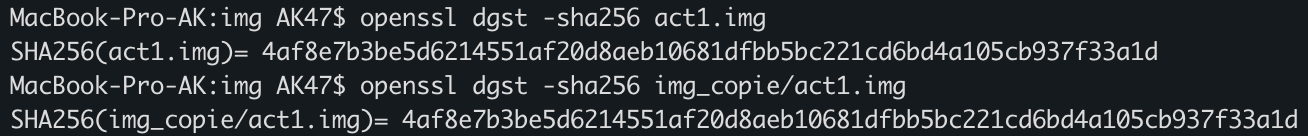
\includegraphics[scale = 0.50]{img/act1/hash.png} 
	\end{center}
	\caption{Cryptographic hash value of act1.img}
	\label{hash}
\end{figure}

\begin{figure}[H]
	\begin{center}
		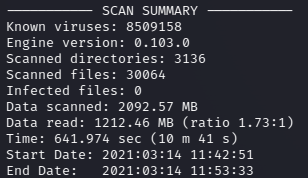
\includegraphics[scale = 0.50]{img/act1/av.png} 
	\end{center}
	\caption{ClamAV result on the act1.img}
	\label{av}
\end{figure}

\begin{figure}[H]
	\begin{center}
		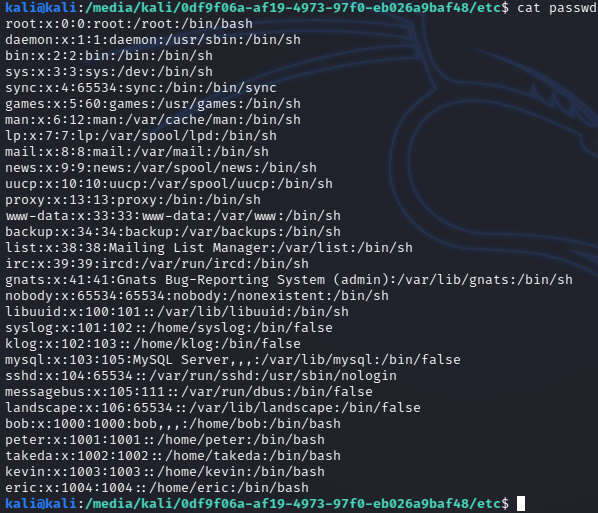
\includegraphics[scale = 0.50]{img/act1/passw.png} 
	\end{center}
	\caption{Passwd file}
	\label{passwd}
\end{figure}

\begin{figure}[H]
	\begin{center}
		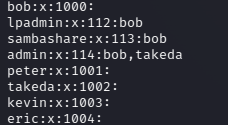
\includegraphics[scale = 0.50]{img/act1/group.png} 
	\end{center}
	\caption{Group file}
	\label{group}
\end{figure}

\begin{figure}[H]
	\begin{center}
		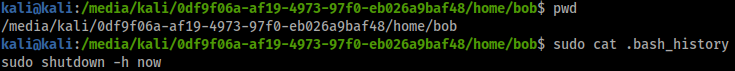
\includegraphics[scale = 0.47]{img/act1/bobHistory.png} 
	\end{center}
	\caption{Bob's Bash History}
	\label{bobBash}
\end{figure}


	
\begin{figure}[H]
	\begin{center}
		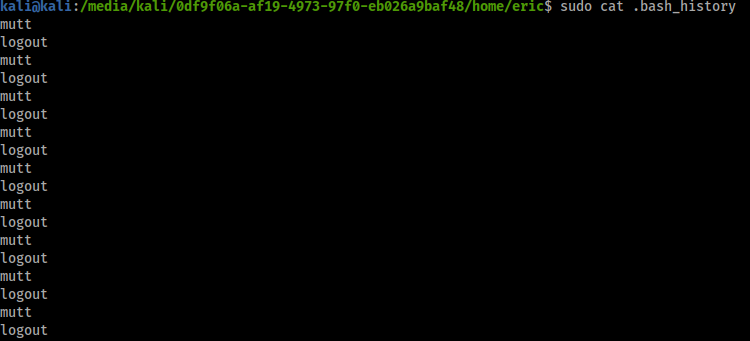
\includegraphics[scale = 0.47]{img/act1/ericHistory.png} 
	\end{center}
	\caption{Eric's Bash History}
	\label{ericBash}
\end{figure}

\begin{figure}[H]
	\begin{center}
		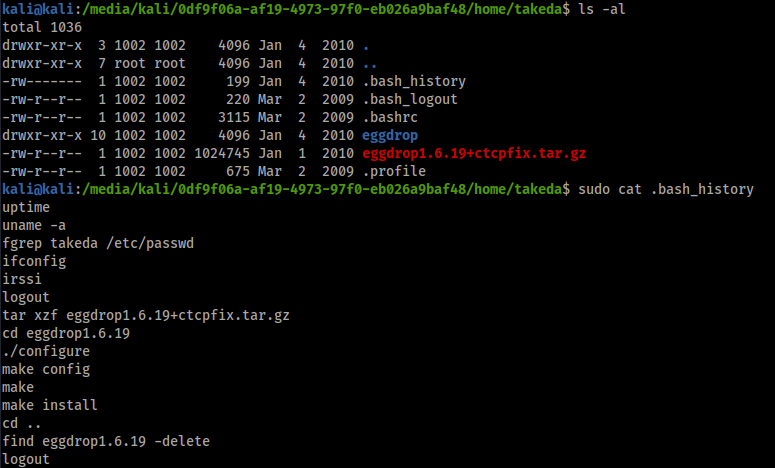
\includegraphics[scale = 0.47]{img/act1/takedaHistory.png} 
	\end{center}
	\caption{Takeda's Bash History + files}
	\label{takedaBash}
\end{figure}


\begin{figure}[H]
	\begin{center}
		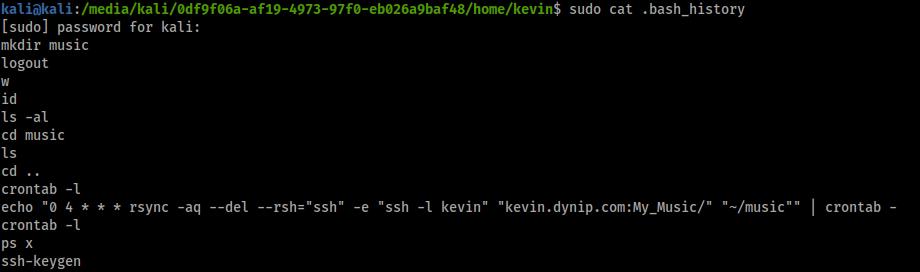
\includegraphics[scale = 0.47]{img/act1/kevinHistory.png} 
	\end{center}
	\caption{Kevin's Bash History}
	\label{kevinBash}
\end{figure}

%----------------------------------

%\begin{figure}[H]
%	\begin{center}
%		\includegraphics[width=350]{Latex_Template/img/er.png} 
%	\end{center}
%	\caption{e2undel command}
%	\label{fig:e2undel}
%\end{figure}


\begin{figure}[H]
	\begin{center}
		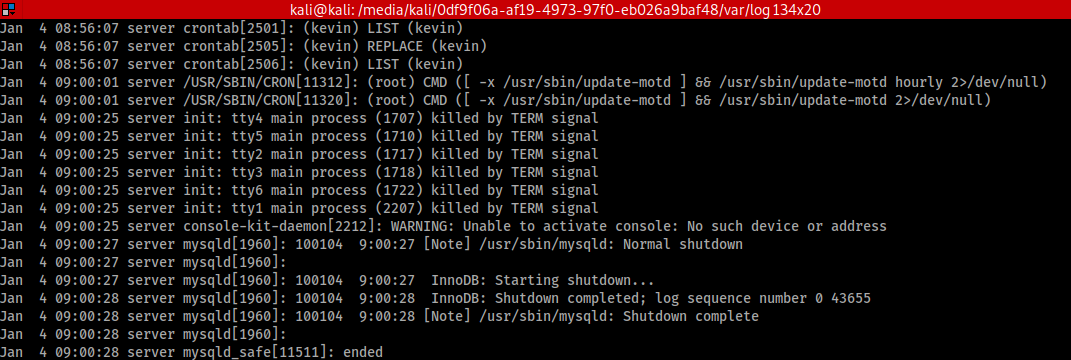
\includegraphics[scale = 0.47]{img/act1/syslog.png} 
	\end{center}
	\caption{Syslog file content}
	\label{syslog}
\end{figure}


\begin{figure}[H]
	\begin{center}
		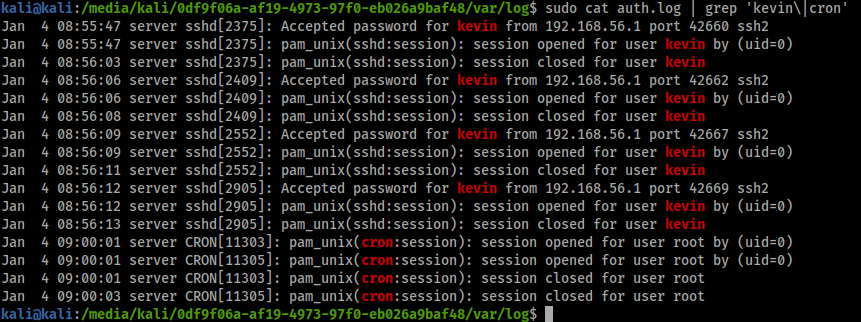
\includegraphics[scale = 0.47]{img/act1/authlogGrep.png} 
	\end{center}
	\caption{Auth.log file content filtered with GREP for kevin and cron}
	\label{authlog}
\end{figure}

\begin{figure}[H]
	\begin{center}
		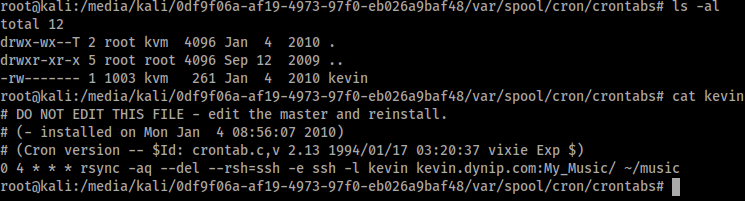
\includegraphics[scale = 0.47]{img/act1/crontab.png} 
	\end{center}
	\caption{Crontab folder with cron file named Kevin}
	\label{crontab}
\end{figure}

\begin{figure}[H]
	\begin{center}
		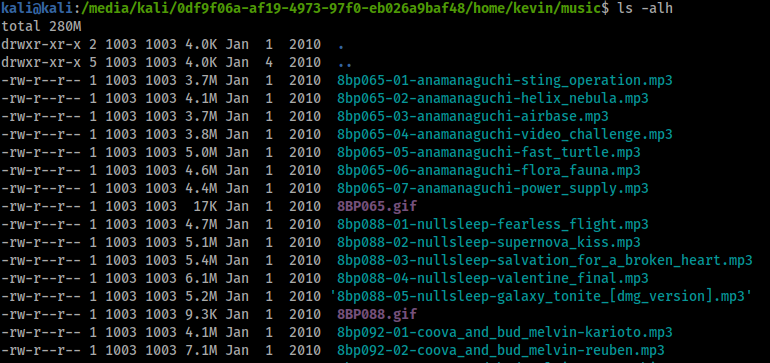
\includegraphics[scale = 0.47]{img/act1/kevinMusic.png} 
	\end{center}
	\caption{Kevin's music folder + total folder's size}
	\label{kevinMusic}
\end{figure}

% Prints your bibliography database xxx.bib
%\bibliographystyle{IEEEtran}
%\bibliography{ref.bib}

\end{document}
